\documentclass[12pt]{article}


% -------------------- PAQUETES --------------------
\usepackage[utf8]{inputenc}
\usepackage[spanish]{babel}
\usepackage[margin=2.54cm]{geometry}
\usepackage{graphicx}
\usepackage{xcolor}


% -------------------- CARGA DE ARCHIVOS EXTERNOS --------------------
% ----------------- UTILIDADES PARA DAR UN MEJOR FORMATO DE DOCUMENTO -----------------  


\definecolor{azul}{rgb}{0.0039, 0.3098, 0.6196}


% Formato para el indice general ...........
\makeatletter
    \renewcommand{\@dotsep}{1.5}
    \renewcommand{\l@section}{\@dottedtocline{1}{1.5em}{2.3em}}
    \renewcommand{\l@subsection}{\@dottedtocline{2}{3.8em}{3.2em}}
    \renewcommand{\l@subsubsection}{\@dottedtocline{3}{7.0em}{4.1em}}
\makeatother

% --------- COMANDOS PERSONALIZADOS PARA LA PORTADA DE LAS TAREAS, TRABAJOS Y PROYECTOS ---------

\newcommand{\rutaLogo}[1]{\newcommand{\RutaLogo}{#1}}
\newcommand{\tema}[1]{\newcommand{\Tema}{#1}}
\newcommand{\etiquetaAutores}[1]{\newcommand{\EtiquetaAutores}{#1}}
\newcommand{\alumno}[1]{\newcommand{\Alumno}{#1}}
\newcommand{\materia}[1]{\newcommand{\Materia}{#1}}
\newcommand{\docente}[1]{\newcommand{\Docente}{#1}}
\newcommand{\ciclo}[1]{\newcommand{\Ciclo}{#1}}
\newcommand{\fecha}[1]{\newcommand{\Fecha}{#1}}
\newcommand{\periodo}[1]{\newcommand{\Periodo}{#1}}



% -------------------- DEFINICIÓN DE LA PORTADA --------------------
\rutaLogo{../../../RecursosGlobales/Img/logo_tec_azuay.png}
\tema{\\ \vspace{1cm} Actividad N°5: Tarea en Clase\\Proposiciones y tablas de verdad \\ \vspace{1.7cm}}
\etiquetaAutores{Alumno:}
\alumno{Eduardo Mendieta \vspace{1cm}}
\materia{Matemática \vspace{1cm}}
\docente{Lcda. Vilma Duchi \vspace{1cm}}
\ciclo{Primer Ciclo \vspace{1.1cm}}
\fecha{10 de junio de 2024 \vspace{1cm}}
\periodo{Abril 2024 - Agosto 2024}



% -------------------- INFORME --------------------
\begin{document}

    \begin{titlepage}

    \centering

    \includegraphics[width=0.11\textwidth]{\RutaLogo} 

    \vspace{0.3cm}
    \textcolor{azul}{\Large \textbf{Instituto Superior Universitario Tecnológico del Azuay \\}}
    \vspace{0.3cm}
    \textcolor{azul}{\Large \textbf{Tecnología Superior en Big Data}}
    
    % 1. ---------------- TEMA -------------------------
    
    {\Large\textbf{\Tema}}
    
    % 2. ---------------- AUTOR(ES) -------------------------
    \textcolor{azul}{\large \textbf{\EtiquetaAutores} \\}
    \vspace{0.3cm}
    {\large \Alumno}

    % 3. ---------------- MATERIA -------------------------
    \textcolor{azul}{\large \textbf{Materia:} \\}
    \vspace{0.3cm}
    {\large \Materia}


    % 3. ---------------- DOCENTE -------------------------
    \textcolor{azul}{\large \textbf{Docente:} \\}
    \vspace{0.3cm}
    {\large \Docente}


    % 3. ---------------- Ciclo -------------------------
    \textcolor{azul}{\large \textbf{Ciclo:} \\}
    \vspace{0.3cm}
    {\large \Ciclo}


    % 3. ---------------- FECHA -------------------------
    \textcolor{azul}{\large \textbf{Fecha:} \\}
    \vspace{0.3cm}
    {\large \Fecha}

    % 3. ---------------- PERIODO -------------------------
    \textcolor{azul}{\large \textbf{Periodo Académico:} \\}
    \vspace{0.3cm}
    {\large \Periodo}
 
\end{titlepage}

  
    \section*{\centering Tarea en Clase - Proposiciones y tablas de verdad}
        \textbf{Formaliza la siguiente proposición y encuentre la tabla de verdad:}

        \begin{enumerate}
             % EJERCICIO 1: ----------------------------------------------------
            \item \textbf{Si tuvieran que justificarse ciertos hechos por su enorme tradición entonces, si estos hechos son inofensivos y respetan a todo ser viviente y al medio ambiente, no habría ningún problema. Pero si los hechos son bárbaros o no respetuosos con los seres vivientes o el medio ambiente, entonces habría que dejar de justificarlos o no podriamos considerarnos dignos de nuestro tiempo.}
                \par$p:$ Justificar ciertos hechos.
                \par$q:$ Los hechos son inofensivos.
                \par$r:$ Los hechos respetan a todo ser viviente.
                \par$s:$ Los hechos respetan al medio ambiente.
                \par$t:$ Existe un problema.
                \par$u:$ Somos dignos de nuestro tiempo.
                \par$n = 6$, $2^n = 2^6 = 64$
                \par\vspace{0.5cm}$p \longrightarrow [((q \wedge r \wedge s) \longrightarrow \sim t) \wedge ((\sim q \vee \sim (r \vee s)) \longrightarrow (\sim p \vee \sim u))]$

            
                \begin{figure}[!h]
                    \centering
                    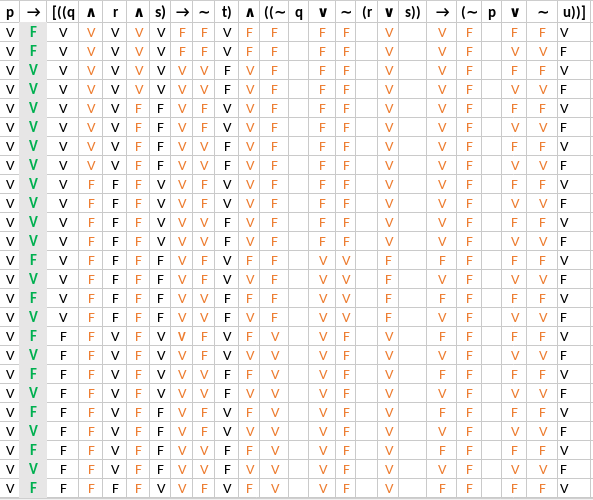
\includegraphics[width=0.6\textwidth]{Img/Tarea5_ej1_1.png}
                \end{figure}

                \newpage
                \begin{figure}[!h]
                    \centering
                    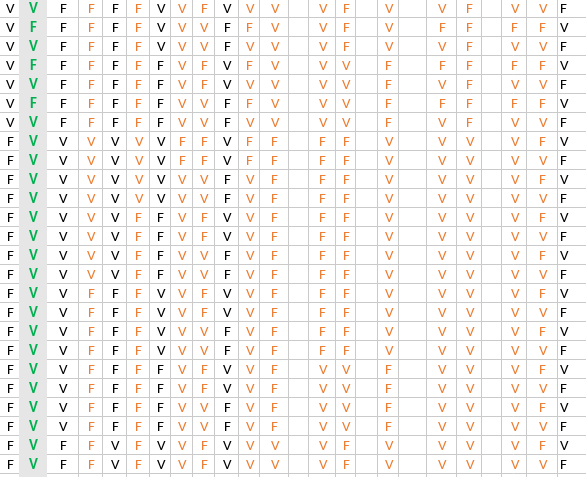
\includegraphics[width=0.6\textwidth]{Img/Tarea5_ej1_2.png}
                \end{figure}

                \begin{figure}[!h]
                    \centering
                    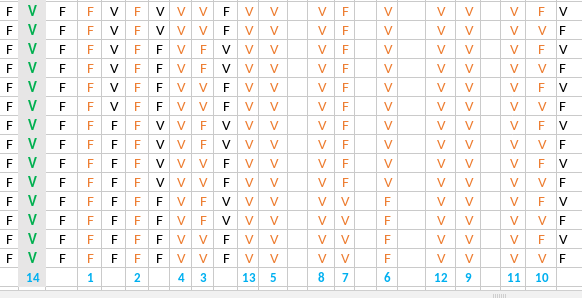
\includegraphics[width=0.6\textwidth]{Img/Tarea5_ej1_3.png}
                \end{figure}

                \textbf{Respuesta:} El enunciado es una contingencia.

        \end{enumerate}

\end{document}